\chapter{Développement et Implémentation}

\section{Structure de la base de données}
La modélisation de la base de données a été réalisée avec une attention particulière portée à la scalabilité et aux performances. Comme le recommande \cite{martin2017clean}, la conception a suivi les principes de normalisation pour éviter la redondance des données.

\begin{figure}[H]
	\centering
	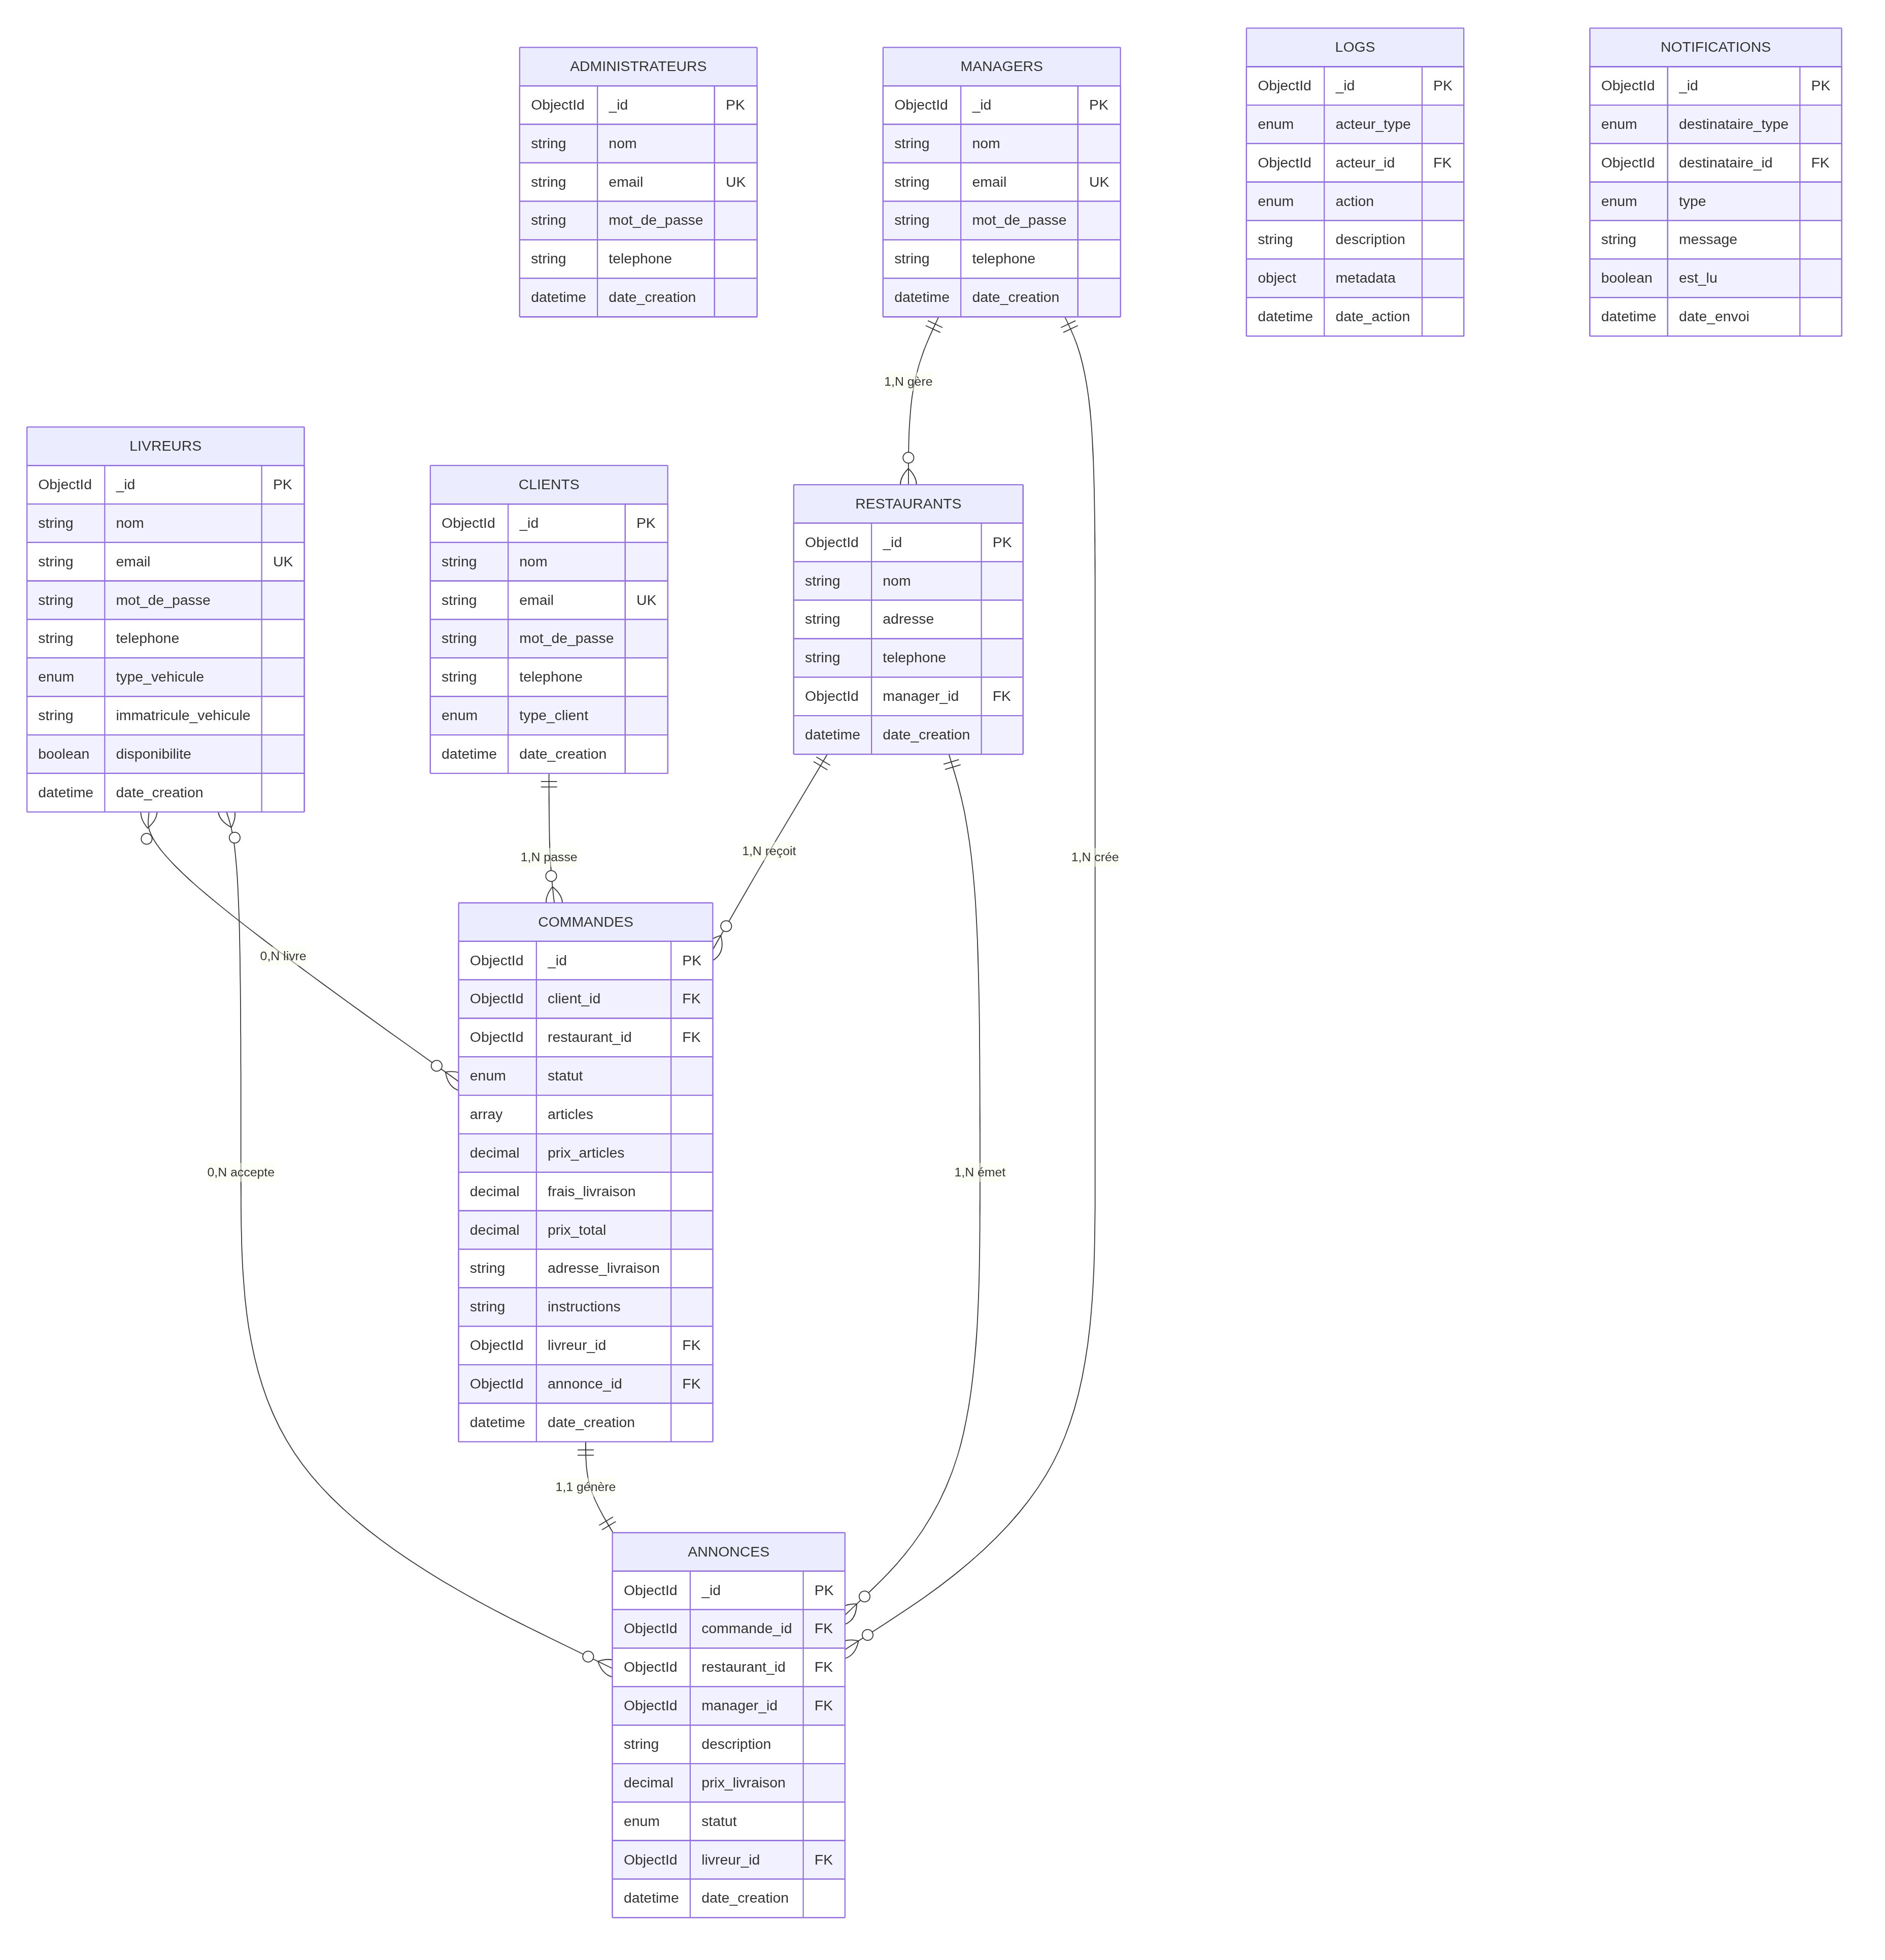
\includegraphics[width=0.9\textwidth]{images/modele-donnees.png}
	\caption{Modèle de données relationnel}
	\label{fig:modele-donnees}
\end{figure}

\subsection{Entités principales}
Le schéma comprend les entités suivantes :
\begin{itemize}
	\item \textbf{User} : Gestion des utilisateurs et permissions
	\item \textbf{Project} : Informations sur les projets
	\item \textbf{Task} : Tâches avec relations parent-enfant
	\item \textbf{TimeEntry} : Suivi du temps par tâche
\end{itemize}

\section{Développement des API}
Les API RESTful ont été développées avec Express.js et documentées avec Swagger. L'implémentation respecte scrupuleusement les contraintes REST définies par \cite{fielding2000rest}, garantissant une API stateless et uniforme.

\subsection{Exemple d'endpoint}
\begin{verbatim}
	// Création d'une tâche
	POST /api/projects/{projectId}/tasks
	{
		"title": "Développer composant login",
		"description": "Créer le composant...",
		"assigneeId": "user-123",
		"dueDate": "2024-07-30"
	}
\end{verbatim}

\section{Interface utilisateur}
Le développement frontend a suivi une approche component-driven avec Storybook pour la documentation des composants. L'utilisation de React \cite{react2024} a permis de créer une interface utilisateur réactive et maintenable.

\begin{table}[H]
	\centering
	\caption{Métriques de qualité du code}
	\begin{tabular}{lccc}
		\toprule
		\textbf{Métrique} & \textbf{Backend} & \textbf{Frontend} & \textbf{Target} \\
		\midrule
		Couverture tests & 85\% & 78\% & >80\% \\
		Complexité cyclomatique & 2.1 & 1.8 & <3 \\
		Dette technique (jours) & 0.5 & 1.2 & <2 \\
		Maintenabilité & A & A & A \\
		\bottomrule
	\end{tabular}
\end{table}

\section{Gestion d'état}
L'état de l'application est géré via une combinaison de :
\begin{itemize}
	\item React Query pour les données serveur, optimisant les performances comme recommandé dans la documentation React \cite{react2024}
	\item Context API pour l'état global client
	\item useState/useReducer pour l'état local
\end{itemize}

L'architecture backend basée sur Node.js \cite{nodejs2024} assure une gestion efficace des requêtes simultanées, tandis que la structure du code suit les principes de \cite{martin2017clean} pour une maintenabilité optimale.